\begin{pastexam}[label={px:ust-112-ee-ds-24}]{臺聯大電機類 112 學年度 第 24 題}
（問答；10 分）

Please construct the minimum spanning tree (MST) for the given graph using Kruskal's Algorithm.
(6 points) What is the weight of the MST? (4 points)

\begin{center}
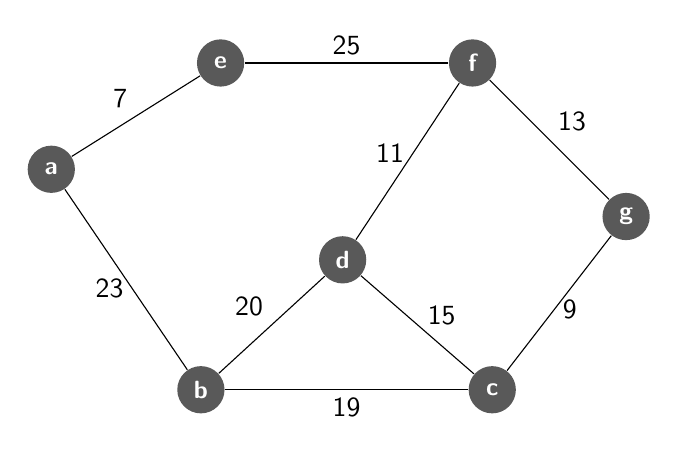
\begin{tikzpicture}[v/.style={circle,fill=black!65,text=white,font=\sffamily\bfseries\small,inner sep=1.5pt,minimum size=6mm},
  w/.style={font=\sffamily,inner sep=3pt}]
\node[v] (a) at (0,0) {a};
\node[v] (e) at (2.15,1.35) {e};
\node[v] (f) at (5.35,1.35) {f};
\node[v] (g) at (7.3,-0.6) {g};
\node[v] (d) at (3.7,-1.15) {d};
\node[v] (b) at (1.9,-2.8) {b};
\node[v] (c) at (5.6,-2.8) {c};
\draw (a) -- node[w,above left] {7} (e);
\draw (e) -- node[w,above] {25} (f);
\draw (f) -- node[w,left,pos=0.45] {11} (d);
\draw (f) -- node[w,above right] {13} (g);
\draw (a) -- node[w,left,pos=0.55] {23} (b);
\draw (b) -- node[w,above left,pos=0.5] {20} (d);
\draw (d) -- node[w,above right,pos=0.55,inner sep=1.5pt] {15} (c);
\draw (b) -- node[w,below] {19} (c);
\draw (g) -- node[w,right,pos=0.55] {9} (c);
\end{tikzpicture}
\end{center}
\end{pastexam}

\begin{pastsoln}
答案：MST 的邊是 $ae$、$gc$、$fd$、$fg$、$bc$、$ab$，權重 $82$。

Kruskal 演算法（資結書第~24.2~節、虛擬碼~24.2）：把邊依權重由小到大排序，依序檢查；兩端點在
不同的元件就加入（並把兩個元件合併），在同一個元件就會成環，捨棄。 $7$ 個頂點的生成樹要 $6$ 條邊。

\begin{center}
\begin{tabular}{cclll}
\toprule
順序 & 邊 & 權重 & 結果 & 加入後的元件／捨棄的理由 \\
\midrule
1 & $ae$ & 7  & 加入 & $\{a, e\}$ \\
2 & $gc$ & 9  & 加入 & $\{a, e\}$、$\{c, g\}$ \\
3 & $fd$ & 11 & 加入 & $\{a, e\}$、$\{c, g\}$、$\{d, f\}$ \\
4 & $fg$ & 13 & 加入 & $\{a, e\}$、$\{c, d, f, g\}$ \\
5 & $dc$ & 15 & 捨棄 & $d$、$c$ 已同一元件，會成環 $d$--$c$--$g$--$f$--$d$ \\
6 & $bc$ & 19 & 加入 & $\{a, e\}$、$\{b, c, d, f, g\}$ \\
7 & $bd$ & 20 & 捨棄 & 會成環 $b$--$d$--$f$--$g$--$c$--$b$ \\
8 & $ab$ & 23 & 加入 & $\{a, b, c, d, e, f, g\}$ \\
\bottomrule
\end{tabular}
\end{center}
加入第 8 條檢查的邊 $ab$ 之後已經有 $6$ 條邊、全部頂點連通，演算法結束；剩下的 $ef = 25$ 不必再看
（看了也會成環）。

MST（粗線）：
\begin{center}
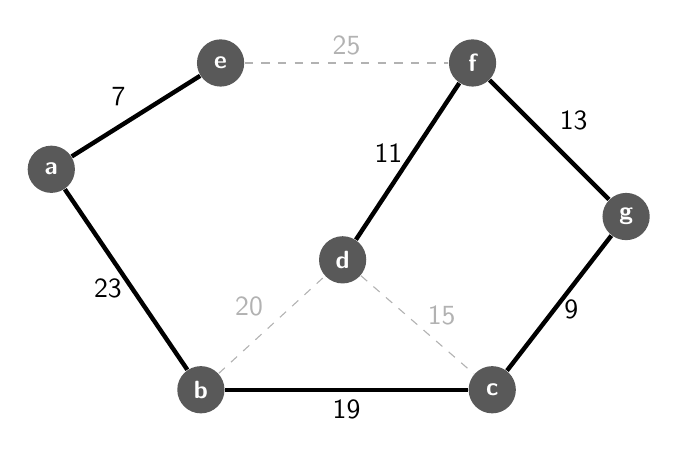
\begin{tikzpicture}[v/.style={circle,fill=black!65,text=white,font=\sffamily\bfseries\small,inner sep=1.5pt,minimum size=6mm},
  w/.style={font=\sffamily,inner sep=3pt}, t/.style={line width=1.6pt}, n/.style={black!30, dashed}]
\node[v] (a) at (0,0) {a};
\node[v] (e) at (2.15,1.35) {e};
\node[v] (f) at (5.35,1.35) {f};
\node[v] (g) at (7.3,-0.6) {g};
\node[v] (d) at (3.7,-1.15) {d};
\node[v] (b) at (1.9,-2.8) {b};
\node[v] (c) at (5.6,-2.8) {c};
\draw[t] (a) -- node[w,above left] {7} (e);
\draw[n] (e) -- node[w,above] {25} (f);
\draw[t] (f) -- node[w,left,pos=0.45] {11} (d);
\draw[t] (f) -- node[w,above right] {13} (g);
\draw[t] (a) -- node[w,left,pos=0.55] {23} (b);
\draw[n] (b) -- node[w,above left,pos=0.5] {20} (d);
\draw[n] (d) -- node[w,above right,pos=0.55,inner sep=1.5pt] {15} (c);
\draw[t] (b) -- node[w,below] {19} (c);
\draw[t] (g) -- node[w,right,pos=0.55] {9} (c);
\end{tikzpicture}
\end{center}
權重 $7 + 9 + 11 + 13 + 19 + 23 = 82$。

所有邊權重都不同，所以 MST 唯一（資結書定理~24.4），用 Prim 或其他方法也會得到同一棵。
\end{pastsoln}
